%%%%%%%%%%%%%%%%%%%%%%%%%%%%%%%%%%%%%%%%%
% Arsclassica Article
% LaTeX Template
% Version 1.1 (1/8/17)
%
% This template has been downloaded from:
% http://www.LaTeXTemplates.com
%
% Original author:
% Lorenzo Pantieri (http://www.lorenzopantieri.net) with extensive modifications by:
% Vel (vel@latextemplates.com)
%
% License:
% CC BY-NC-SA 3.0 (http://creativecommons.org/licenses/by-nc-sa/3.0/)
%
%%%%%%%%%%%%%%%%%%%%%%%%%%%%%%%%%%%%%%%%%

%----------------------------------------------------------------------------------------
%	PACKAGES AND OTHER DOCUMENT CONFIGURATIONS
%----------------------------------------------------------------------------------------

\documentclass[
10pt, % Main document font size
a4paper, % Paper type, use 'letterpaper' for US Letter paper
oneside, % One page layout (no page indentation)
%twoside, % Two page layout (page indentation for binding and different headers)
headinclude,footinclude, % Extra spacing for the header and footer
BCOR5mm, % Binding correction
]{scrartcl}
\usepackage{enumitem}% http://ctan.org/pkg/enumitem

\newcommand\ytl[2]{
	\parbox[b]{8em}{\hfill{\color{cyan}\bfseries\sffamily #1}~$\cdots\cdots$~}\makebox[0pt][c]{$\bullet$}\vrule\quad \parbox[c]{10cm}{\vspace{7pt}\color{red!40!black!80}\raggedright\sffamily #2.\\[7pt]}\\[-3pt]}
\usepackage{tabularx}


\usepackage[]{biblatex}
\addbibresource{sample.bib}

\usepackage[pdftex,
pdfauthor={Andrea Bellani},
pdftitle={UppaalTD: a Formal Tower Defense Game (report)},
pdfsubject={Formal methods for concurrent and real-time systems},
pdfkeywords={Formal methods, concurrent systems, real-time systems, Uppaal, Politecnico di Milano},
pdfproducer={Latex with hyperref},
pdfcreator={pdflatex}]{hyperref}

%%%%%%%%%%%%%%%%%%%%%%%%%%%%%%%%%%%%%%%%%
% Arsclassica Article
% Structure Specification File
%
% This file has been downloaded from:
% http://www.LaTeXTemplates.com
%
% Original author:
% Lorenzo Pantieri (http://www.lorenzopantieri.net) with extensive modifications by:
% Vel (vel@latextemplates.com)
%
% License:
% CC BY-NC-SA 3.0 (http://creativecommons.org/licenses/by-nc-sa/3.0/)
%
%%%%%%%%%%%%%%%%%%%%%%%%%%%%%%%%%%%%%%%%%

%----------------------------------------------------------------------------------------
%	REQUIRED PACKAGES
%----------------------------------------------------------------------------------------

\usepackage[
nochapters, % Turn off chapters since this is an article        
beramono, % Use the Bera Mono font for monospaced text (\texttt)
eulermath,% Use the Euler font for mathematics
pdfspacing, % Makes use of pdftex’ letter spacing capabilities via the microtype package
dottedtoc % Dotted lines leading to the page numbers in the table of contents
]{classicthesis} % The layout is based on the Classic Thesis style

\usepackage{arsclassica} % Modifies the Classic Thesis package

\usepackage[T1]{fontenc} % Use 8-bit encoding that has 256 glyphs

\usepackage[utf8]{inputenc} % Required for including letters with accents

\usepackage{graphicx} % Required for including images
\graphicspath{{Figures/}} % Set the default folder for images

\usepackage{enumitem} % Required for manipulating the whitespace between and within lists

\usepackage{lipsum} % Used for inserting dummy 'Lorem ipsum' text into the template

\usepackage{subfig} % Required for creating figures with multiple parts (subfigures)

\usepackage{amsmath,amssymb,amsthm} % For including math equations, theorems, symbols, etc

\usepackage{varioref} % More descriptive referencing
\usepackage[left=2cm,right=2cm,top=2cm,bottom=1.5cm]{geometry}

%----------------------------------------------------------------------------------------
%	THEOREM STYLES
%---------------------------------------------------------------------------------------

\theoremstyle{definition} % Define theorem styles here based on the definition style (used for definitions and examples)
\newtheorem{definition}{Definition}

\theoremstyle{plain} % Define theorem styles here based on the plain style (used for theorems, lemmas, propositions)
\newtheorem{theorem}{Theorem}

\theoremstyle{remark} % Define theorem styles here based on the remark style (used for remarks and notes)

%----------------------------------------------------------------------------------------
%	HYPERLINKS
%---------------------------------------------------------------------------------------
 % Include the structure.tex file which specified the document structure and layout


\hyphenation{Fortran hy-phen-ation} % Specify custom hyphenation points in words with dashes where you would like hyphenation to occur, or alternatively, don't put any dashes in a word to stop hyphenation altogether

\title{\normalfont\spacedallcaps{UppaalTD: a Formal Tower Defense Game}} % The article title

\subtitle{Formal Methods for Concurrent and Real-Time Systems Homework} % Uncomment to display a subtitle

\author{\spacedlowsmallcaps{Andrea Bellani} (\href{mailto:andrea1.bellani@mail.polimi.it}{\nolinkurl{andrea1.bellani@mail.polimi.it}})}

\date{\today} % An optional date to appear under the author(s)



\begin{document}
	
	\renewcommand{\sectionmark}[1]{\markright{\spacedlowsmallcaps{#1}}}
	\lehead{\mbox{\llap{\small\thepage\kern1em\color{halfgray} \vline}\color{halfgray}\hspace{0.5em}\rightmark\hfil}}
	
	\pagestyle{scrheadings} % Enable the headers specified in this block
	
	\maketitle % Print the title/author/date block
	
	\paragraph*{Abstract}
		Uppaal is a tool for modeling, simulating and verifying real-time system as networks of timed automatons. In this report, we present our modeling and verification of the game UppaalTD (both vanilla and stochastic versions) in Uppaal. In Addition, we also analyze the model behavior with selected configurations and define metrics to compare them.
		
	\setcounter{tocdepth}{3} % Set the depth of the table of contents to show sections and subsections only
	
	\tableofcontents % Print the table of contents
	
	\listoffigures % Print the list of figures
	
	\listoftables % Print the list of tables
	
	\newpage
	
	\section{Introduction}
		\subsection{Definitions}
			\begin{itemize}
				\item \textbf{requirements} : the official specifications of UppaalTD's parameters and rules;
				\item \textbf{alive}, \textbf{targettable} or \textbf{shootable} enemy : the enemy has an health strictly greater than zero and is present on the map;
				\item \textbf{dismissed} enemy : the enemy is dead or it shot the MT and the following delay has expired;
				\item \textbf{ending} of a wave : a wave is considered \emph{ended} when each enemy is dismissed (i.e. it can't move or shoot anymore because it has already shoot or it was killed by turrets);
				\item \textbf{winning} configuration : in Vanilla version, a configuration is winning if, by setting it, a wave of 3 circles and 3 square can never defeat the MT. In addition, we define also this terminologies (for Vanilla version with 3 circles and 3 squares):
					\begin{itemize}
						\item \textbf{weakly-winning} configuration : a configuration that does not let the MT to be defeated in at least one game execution;
						\item \textbf{strongly-winning} configuration : a configuration that does not let the MT to be damaged in any game execution;
						\item \textbf{weakly-strongly-winning} configuration : a configuration that does not let the MT to be damaged in at least one game execution;
					\end{itemize}
				\item \textbf{location} : a location of an Uppaal template;
				\item \textbf{state} : the entire game's state in a certain time instant (i.e. each automaton's position and each variable's or clock's value);
				\item \emph{Chebyshev distance} : given two generic $n$-dimensional points $x=(x_1 \dots x_n)$ and $y=(y_1 \dots y_n)$, their Chebyshev distance can be computed as $\max\limits_{1\leq i\leq n}\{|x_i - y_i|\}$.
			\end{itemize}					
		\subsection{Project development timeline}
			\begin{table}[h!]
				\centering
				\begin{minipage}[h!]{.8\linewidth}
					\color{gray}
					\rule{\linewidth}{1pt}
					\ytl{april 8th}{First brief analysis of the requirements}
					\ytl{april 9th}{Uppaal and homework presentation}
					\ytl{april 11th}{First definition of channels and MT's template}
					\ytl{april 26th}{First definition of enemy and turret template (still not synchronized) and shoot to MT modeled with \texttt{STMTCONTROLLER}}
					\ytl{may 1st}{Complete definition of all templates and synchronization without \texttt{STMTCONTROLLER}}
					\ytl{may 15th}{First definition of queries}
					\ytl{may 17th}{Enemy compact version}
					\ytl{may 24th}{Re-design of synchronization with clocks}
					\ytl{june 15th}{First stochastic version}
					\ytl{june 24th}{Started delivery procedures}
					\ytl{june 26th}{Started report writing}
					\ytl{july 14th}{Finished report writing}
					\bigskip
					\rule{\linewidth}{1pt}%
				\end{minipage}
				\caption{Project development timeline}
			\end{table}
		\subsection{Document structure}
			Main sections:
			\begin{enumerate}
				\item \textbf{Introduction} : sum up of our definitions for the terminologies used in the document and project development timeline;
				\item \textbf{Model description} : description of the models with focus on the most critical modeling choices;
				\item \textbf{Verification results} : detailed analysis of the queries verified;
				\item \textbf{Analysis of selected configurations} : presentation and deeper analysis of the models behaviors for some interesting configurations;
				\item \textbf{Conclusions} : resume of the results obtained.
			\end{enumerate}
			Appendixes:
			\begin{enumerate}
				\item[A] \textbf{Discarded choices} : presentation of the most interesting discarded design choices and the motivations behind their rejection.
			\end{enumerate}
		\subsection{Software and machines used}
			\begin{table}[h!]
				\centering
				\begin{tabular}{lll}
					\toprule
					Usage     & Software & Versioning   \\
					\midrule
					Modeling, simulation and verification & Uppaal & 5.0.0  \\
					\addlinespace
					Report writing & TeXstudio & 4.6.3 \\
					\addlinespace
					Versioning  & Git & 2.40.0.windows.1  \\
					\addlinespace
					Configurations drawing & draw.io & v28.0.4  \\
					\bottomrule
				\end{tabular}
				\caption{Software used}
			\end{table}
			Each query was verified on two different machines with different hardware and performances:
			\begin{table}[h!]
				\centering
				\begin{tabularx}{\textwidth}{>{\raggedright\arraybackslash}p{2.5cm} >{\raggedright\arraybackslash}p{3.5cm} >{\raggedright\arraybackslash}p{3.5cm} >{\raggedright\arraybackslash}p{3cm} >{\raggedright\arraybackslash}p{2.5cm}}
					\toprule
					Machine name & CPU & RAM & OS & Manufacturing year\\
					\midrule
					\textbf{Machine 1} & AMD Ryzen 5 3500U (2.1 GHz)  & 8 GB (5,95 GB usable) & Windows 11 Home & 2020  \\
					\addlinespace
					\textbf{Machine 2} & 11th Gen Intel(R) Core(TM) i5-1135G7 (2.4 GHz) & 24 GB (23,7 GB usable) & Windows 11 Pro & 2021\\
					\bottomrule
				\end{tabularx}
				\caption{Machines specifications}
			\end{table}
			
			This document was written over the template Arsclassica Article (\url{https://www.latextemplates.com/template/arsclassica-article}) with few adjustments by us.
	\newpage
	\section{Model description}
		We modeled both the Vanilla and the Stochastic version of the game. In particular, we firstly modeled the Vanilla version and then proceeded to modify it to model the stochastic requirements. In this section we provide a detailed explanation of both versions and how the Stochastic one was obtained from the Vanilla one..
		\subsection{Entities modeling (for Vanilla version)}
			\subsubsection{Map}
				There is no template that models the Map. Each enemy and each turret has a \texttt{Cell} variable that represents its actual position on the map (\texttt{Cell} is simply a \texttt{struct} with two bounded integers):
				\begin{itemize}
					\item an enemy keeps its position updated while moving with the function \texttt{next}. If an enemy is outside of the map (because it has not spawned yet or it was dimissed) its position still has a "feasible" value but a flag prevents turrets to read it (see the following sections for more details);
					\item a turret can't change its position, it simply uses it to calculate its distance from enemies.  
				\end{itemize}
				To be clear, red paths structures are "embedded" into the function \texttt{next}. Another possibility (implemented in some of the previous versions) would have been to define a \texttt{Cell} matrix (or vectors) instead of defining the entire structure as a sequence of if-else in \texttt{next}. We preferred the latter since \texttt{next} is constant in time and space however, with a more complex map, this approach could result in a too difficult to maintain solution.
			\subsubsection{Main Tower (MT)}
				There is no template that models the Main Tower, it is simply modeled as a variable that enemies decrement in the shot. Originally, an MT template was designed (see the appendix for more details), it was removed in an attempt of optimizing the model, since we understood (after reasoning more on other more crucial design choices) that a so simple and "passive" entity like the MT does not really need to be implemented with a dedicated template.
				
				Decoupling enemy and turret in two templates is necessary to model in a proper and clear way the interleaving between these entities but MT neither needs to trigger other components nor has any non-deterministic behavior. The only one centralized aspect that a dedicated template could have implemented was controlling that MT's life is not $0$ before decreasing it, but this can be easily moved in enemy's template (before an enemy shoots, it checks that MT's life is not $0$) without loss of readability.
			\subsubsection{Enemy}
				\begin{flushleft}
					\textbf{Spawn of an enemy}
					
					To model the requirement that circles spawn "every x time units" and squares spawn "every y time units" we simply added a parameter \texttt{spawningTime} to the enemy template. This parameter is simply a delay that must first elapse before an enemy can spawn on the map. By setting it (when we instantiate enemy processes) to \texttt{id$\times$s} (where \texttt{s} is the spawning time defined for that kind of enemy in the requirements), the enemy with id $0$ will spawn in the first time unit, the one with id $i$ will spawn with a delay of \texttt{s} time units and so on:
					\begin{table}[h!]
						\centering
						\begin{tabular}{rcccccc}
							% Prima riga senza bordi
							& circle(0) & \dots & circle(M-1) & square(M) & \dots & square(N-1) \\
							id: & 0 & \dots & M-1 & M & \dots & N-1\\
							\texttt{spawningTime}: & 0 & \dots & 2$\times$(M-1) & 0 & \dots & 3$\times$(N-1-M) \\
						\end{tabular}
						\caption{\texttt{spawningTime} assignment (using requirements spawning times)}
					\end{table}
				\end{flushleft}
				\begin{flushleft}
					\textbf{Initialization of an enemy} (this paragraph aims only to group all the aspects related to the enemy template that will be explained further)
					
					Once an enemy is spawned, it has to:
					\begin{itemize}
						\item initialize its record in the \texttt{shoot\_table} and update the counter of targetable enemies;
						\item reset the \texttt{trip\_time} clock;
						\item set \texttt{chosenPath}.
					\end{itemize}
				\end{flushleft}
				\begin{flushleft}
					\textbf{Move of an enemy}
					
					After the speed delay has expired, an enemy has to make a move. In fact, a move is simply an update of the enemy's position with the function \texttt{next} and a consequent update of the \texttt{shoot\_table} record (see the communication section).
					
					The very interesting design choice behind the move of an enemy is how a (deterministic, since Uppaal \texttt{random} is not available in symbolic simulation) function like \texttt{next} can model the non-deterministic next cell choice an enemy has to take in a red paths junction. Simply, the choices an enemy will take in junctions are non-deterministically determined "a priori" when an enemy spawns, by calling \texttt{initialize} with different parameters:
					\begin{figure}[h!]
						\centering
						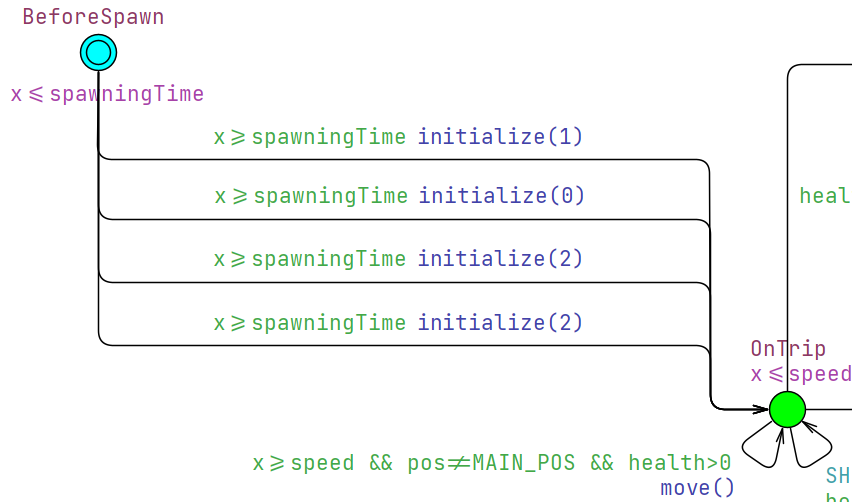
\includegraphics[width=0.55\textwidth]{ndPathChoice.png}
						\caption{Close-up of how "a priori" non-deterministic path choice is implemented in the enemy template}
					\end{figure}
					
					We realized that since during the game there is no event that may change the probability that an enemy takes a certain choice in a junction rather than another, without loss of generality these non-deterministic choices can be determined all at once by the time the enemy spawns.
					
					This simple intuition really improved the readability of the enemy template (in the project development timeline we called this new version \emph{compact enemy}) however, it can be convenient only if there are few possible choices.
					
					Note that even if there exist three possible paths, it would be incorrect to model only one transition per-path. These transitions must model the same probability of taking any "sequence of choices". In other words, the probability of taking the choice "under" in the junction (7,4) has a $0.5$ of probability to be taken, the other $0.5$ is the probability of choosing "up" and then there is a $0.5$ probability for each choice in the junction (10,7). If we want to determine these choices "a priori", it is not correct to model any possible path with a single transition, because it would lead the probability of taking any path to $\frac{1}{N}$ (where $N$ is the number of possible paths to the MT).
				\end{flushleft}
				\begin{flushleft}
					\textbf{Dismissal of an enemy}
					
					Once an enemy has to leave the map, it simply updates properly the \texttt{shoot\_table} record, the counter of the targetable enemies and the counter of the left enemies.
					
					A match is considered ended if the counter of left enemies is zero (i.e. all enemies spawned and leaved the map for a certain reason). Once the enemy is dismissed, it goes in a location where it waits that the match ends and then goes (in the sense that a self-loop with is enabled) in an endless self-loop, this choice is in fact more crucial than it might seem:
					\begin{itemize}
						\item it prevents the system deadlock once the match is ended;
						\item putting a self-loop with no guard would of course prevent deadlocks but it would possibly lead the starvation of other entities since an enemy may arrive in the Dismissed location and then self-looping indefinitely so other entities could not move/shoot anymore, and so preventing some queries to be verified (e.g. query Q2). With the guard, this situation may happen only once all enemies are dismissed (and so no entity can "starve" anymore).
					\end{itemize}
				\end{flushleft}
			\subsubsection{Turret}
				The high-level behavior of a turret (for the design of the communications see the following section) is pretty simple:
				\begin{enumerate}
					\item the turret (in the initial location) is ready to shoot to an enemy as soon as one of them gets into its shooting range (purpose of the function \texttt{canShoot}). It checks other enemies positions by looking into \texttt{shoot\_table};
					\item once \texttt{canShoot} returns true the transition to shoot to an enemy is enabled. If it is performed, the function \texttt{target} selects the nearest enemy in the shooting range (in case of ties it follows the requirements rules), and with \texttt{shoot} the enemy is shot by putting in the global variable \texttt{target\_record} the id of the target and the related damage;
					\item once the shot is performed, the turret waits the delay and then comes back to the initial location.
				\end{enumerate}
				\texttt{canShoot} and \texttt{target} are optimized to avoid useless scans of the \texttt{shoot\_table}, in particular:
				\begin{itemize}
					\item \texttt{canShoot} :
						\begin{itemize}
							\item does not select the enemy to target but simply checks that there is at least one enemy in the shooting range (\texttt{target} has targeting purpose), which is average less complex (but not asymptotically);
							\item while scanning the \texttt{shoot\_table} it keeps counting how many targetable enemies are found (i.e. enemies that are alive on the map), so it can stop as soon as it recognizes that no targetable enemies can be found in the following records;
						\end{itemize}
					\item \texttt{target} :
						\begin{itemize}
							\item scans \texttt{shoot\_table} to find the first targetable enemy in the shooting range. It is considered as the candidate enemy for the shot and the following records are scanned to find a possibly "better" enemy to shoot;
							\item the scan is always stopped as soon as no targetable enemies can be found in the following records.
						\end{itemize}
				\end{itemize}
				Note that the complexity of both \texttt{canShoot} and \texttt{target} is linear in the \texttt{shoot\_table} length but it is totally independent of the size of the shooting range.
				
				Another improvement that could be argued is to let \texttt{canShoot} pass the first enemy in the shooting range found to \texttt{target}, in this way the latter has already a candidate enemy. However, since \texttt{canShoot} is inside a guard, it must be side-effects free, therefore it can't change a value outside of its scope.
		\subsection{Communication modeling description (for Vanilla version)}
			\subsubsection{How turrets shoot to enemies}
				Each enemy has a record in the \texttt{shoot\_table} structure that keeps updated. This record contains all the information turrets need to identify which enemy shoot (position, time in which the enemy spawned and enemy's kind) and a flag to know if that enemy is present on the map.
				
				Once an enemy is targeted, the turret places on the global variable \texttt{target\_record} the id of the target and the related damage. In the meantime a message to all (targetable) enemies is sent over the broadcast channel \texttt{SHOOT\_TO\_ENEMY}, then each one checks if their id corresponds to the one of the target and if it is, they decrement their life accordingly to the damage and in case their health is now zero or below they leave the map.
				
				An important design choice is that \texttt{SHOOT\_TO\_ENEMY} is an urgent channel. In our vision of the game, when a turret can shoot, time can't elapse. This does not avoid situations where the delay of an enemy is fully elapsed and the move is performed while the "urgent" transition is enabled by a turret (because in this case the delay has already fully elapsed, so this update does not concern time) but avoids situations where a turret is ready to shoot and it is completely ignored by the progress of time. In other words, a shot to an enemy must be performed in the same time unit where it is "calculated", any other action that "would make the time progress" is "postponed" as long as the turret can fire. It is a simple rule to extremely reduce the space of possible executions (since transitions related to a shot can never "interleave" the passage of time) and ensure a more predictable and reasonable behavior of the model. We can rephrase this choice by considering time as a resource that enemies need to move and turrets need to shoot. Once a turret is able to shoot, it is not fair (for our interpretation of the game) that time is "gained" by enemies which delay has not fully elapsed yet. Note that this choice can be also interpreted as the opponent case where a turret needs to wait and an enemy can move. In this situation, time can never pass since it is "blocked" by the combination of invariant and guard in the enemy template. Therefore, it would not be fair for turrets if a turret is ready to shoot but enemies (with a delay that still has to elapse) can "ignore" this situation. Note that (this is a more technical explanation) this "fairness" needs \texttt{SHOOT\_TO\_ENEMY} to be urgent since the transition fired once the turret delay has expired is not the one that performs the shoot (since \texttt{canMove} may not be true by the time the delay expires, this design choice may cause deadlocks), in that case we obtained the same effect with an urgent channel.
			\subsubsection{How enemies shoot to the MT}
				Since there is no template for the MT, there is apparently no need to use define a channel to "synchronize" the shot since it is nothing more than a decrement of a global variable. However, we still designed an urgent broadcast channel to guarantee that once an enemy can shoot to the MT, time can't elapse (for the same reason why \texttt{SHOOT\_TO\_ENEMY} is urgent). Note that it is necessary to define the channel as broadcast otherwise, since there is no entity that "receives" the message sent over it, a deadlock would happen if an enemy wants to send a message over a non-broadcast channel where no entity is listening on and the time is blocked since the channel is urgent.
		\subsection{Enrichment of Vanilla model with stochastic features}
			To model the stochastic features, there are no big changes from the Vanilla model but they are crucial:
			\begin{itemize}
				\item enemies and turrets "speeds" delays : it is no more modeled with a clock but with a simple self-transition (which guard of course does not involve clocks) and a \texttt{rate of exponential} properly set to in the location. In this way, the probability of leaving from the state with the self-transition determines the delay before an enemy's move or a turret can shoot again;
				\item self-loop in \texttt{Dismissed} : [SPIEGARE COME MAI DAVVERO E' STATO RIMOSSO, DATO CHE NON CREDO NON SIA CONCESSO AVERE NESSUNO STATO SENZA INVARIANTI E SENZA RATE OF EXPONENTIAL].
			\end{itemize}
			The only delay that is still implemented as a "non-probabilistic" delay is the one related to the spawning time.
			
			Note that there was no change in communication channels since all of them were broadcast also in the Vanilla version (stochastic models can only use broadcast channels) and the motivations behind making them \texttt{urgent} are independent of the stochastic nature of the model.
	\section{Verification results}
		\subsection{Vanilla model verification}
			\subsubsection{Verification without turrets}
				To verify the requested query we wrote the following Uppaal queries:
				\begin{table}[h!]
					\centering
					\begin{tabularx}{\textwidth}{||c|>{\raggedright\arraybackslash}X|>{\raggedright\arraybackslash}X|>{\raggedright\arraybackslash}X|>{\raggedright\arraybackslash}X|>{\raggedright\arraybackslash}X||}
						\hline
						 & Verified properties & Result [T/F] & Verification time on Machine 1 [s] & Verification time on Machine 2 [s] & Average maximum past-waiting list load \\
						\hline
						Q1 & I & T& $\approx$ 9.7 & & $\approx$ 13100\\ \hline
						Q2 & II & T&  $\approx$ 10.5 & & $\approx$ 220\\ \hline
						Q3 & III, IV & T&  $\approx$ 7.3& & $\approx$ 14000\\ \hline
						Q4 & V & T&  $\approx$ 6.8& & $\approx$ 14000\\
						\hline
					\end{tabularx}
					\caption{Queries without turrets overview}
				\end{table}
				Q1 must verify that the system never reaches a deadlock state, our query is then simply:
				\begin{center}
					[METTERE QUERY IN TCTL]
				\end{center}
				Originally, this query aimed only to verify deadlock avoidance only when the match is not ended. In fact, our model can still verify this query if we remove the self-loop on \texttt{Dismissed}. Informally, we can also argue that no deadlocks can happen even in this way: all enemies will eventually become \texttt{Dismissed} all together. Since once all enemies are \texttt{Dismissed} they start the to indefinitely take the self-loop:
				\begin{center}
					[MAGARI METTERE ANCHE QUESTA QUERY IN TCTL]
				\end{center}
				
				Q2 aims to verify that all enemies can reach the MT spot:
				\begin{center}
					contenuto...
				\end{center}
				We interpreted "can reach" in the sense that in any possible path all enemies will reach the MT, this is the reason way this query is not stated with "E...".
				
				Another important motivation behind this formulation is that this query in reality verifies that exists state in any possible path where all enemy have their position in the MT spot all together. This condition is easy to guarantee in our model since the dismissal of an enemy keeps \texttt{pos} to the last value it had right before the dismissal. It is like we are "freezing" in the \texttt{pos} the fact that the enemy reached the MT spot, but at the end the model will permit to any enemy to reach the MT spot.
				
				Q3 verifies both that each circle and each square satisfy the time constraint:
				\begin{center}
					[METTERE QUERY IN TCTL]
				\end{center}
				Simply once an enemy is \texttt{OnTrip} and reaches the MT spot, it must have satisfied the time constraint for its kind. \texttt{trip\_time} is a classic clock that counts the time units passed from the initialization (i.e. the time unit when the enemy spawned).
				
				Note that this query would not be satisfied in this form if \texttt{SHOOT\_TO\_MT} was not \texttt{urgent}, since this property imposes that time (and so also \texttt{trip\_time}) can't progress as long as the MT spot in reached in \texttt{OnTrip}.
				
				Q4 is probably the most intuitive query:
				\begin{center}
					[METTERE QUERY IN TCTL]
				\end{center}
				In any state of any possible path, if an enemy is targetable it must be on a red spot.
				
				Note that since \texttt{pos} is by default \texttt{{0,0}} before spawning and it is kept to the MT spot once it is reached, even if an enemy is not targetable anymore it will anyway be in a red spot. We put this restriction to the "query scope" because there is no need to check \texttt{pos} if an enemy is not present on the map. 
			\subsubsection{Verification with turrets}
				To verify the requested query we wrote the following Uppaal queries:
				\begin{table}[h!]
					\centering
					\begin{tabularx}{\textwidth}{||c|>{\raggedright\arraybackslash}X|>{\raggedright\arraybackslash}X|>{\raggedright\arraybackslash}X|>{\raggedright\arraybackslash}X|>{\raggedright\arraybackslash}X||}
						\hline
						& Verified properties & Result [T/F] & Verification time on Machine 1 [s] & Verification time on Machine 2 [s] & Average maximum past-waiting list load \\
						\hline
						Q1 & VII & T & $\approx$ 284.3 & & $\approx$ 50000\\ \hline
						Q5 & VI & T &  $\approx$ 100.4 & & $\approx$ 49000  \\
						\hline
					\end{tabularx}
					\caption{Queries with turrets overview}
				\end{table}
				
				Q1 is used also for verifying VII since the total absence of deadlocks, in symbolic simulation, can be stated by means of the keyword \texttt{deadlock}.
				
				Since we defined a "winning" configuration as a configuration that can never let the MT to be defeated by a wave of six (three circles and three squares) enemies, a query that is true if and only if a configuration is winning is:
				\begin{center}
					mettere query in TCTL
				\end{center}
				If the MT is defeated in at least one state of one path, the query will not be satisfied (with the configuration chosen).
				
				Note that in the configurations section we also analyze the other kinds of "winning" of them. For brevity, we do not report those queries but they are really similar to Q1 (e.g. to verify the weakly-winning property, it is sufficient to verify the query [METTERE QUERY IN TCTL]).
		\subsection{Stochastic model verification}
	\newpage
	\section{Analysis of selected configurations}
		\subsection{Vanilla version}
			We further analyzed the default configuration with turrets and four more configurations:
			\begin{figure}[h!]
				\centering
				\begin{minipage}{.4\textwidth}
					\centering
					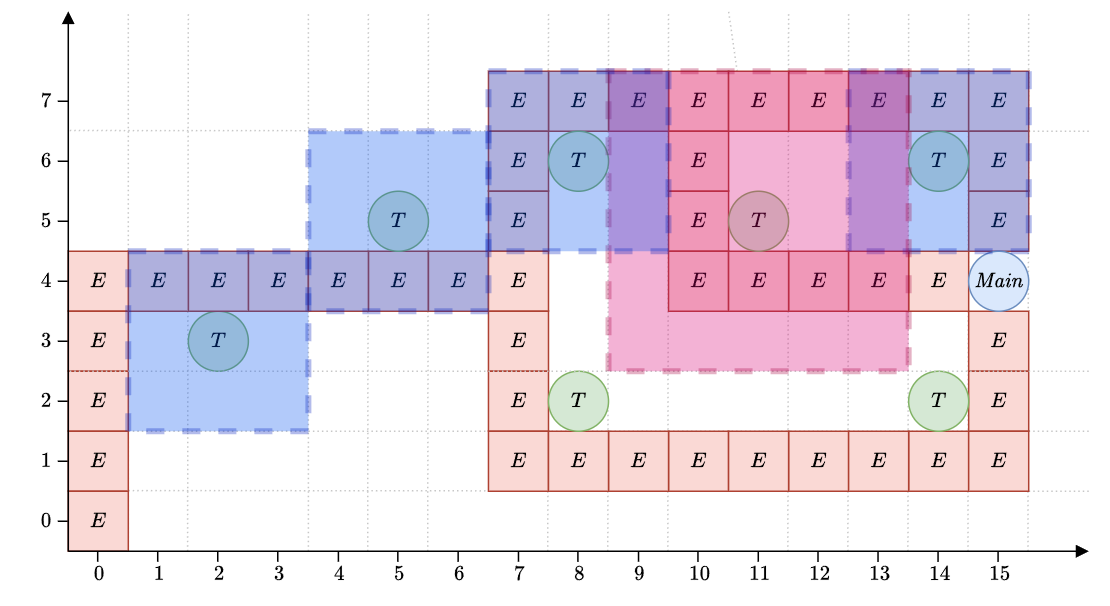
\includegraphics[width=\linewidth]{configs/vanilla/DownFromCannons.png}
					\caption{\emph{DownFromCannons} configuration}
				\end{minipage}
				\begin{minipage}{.5\textwidth}
					\centering
					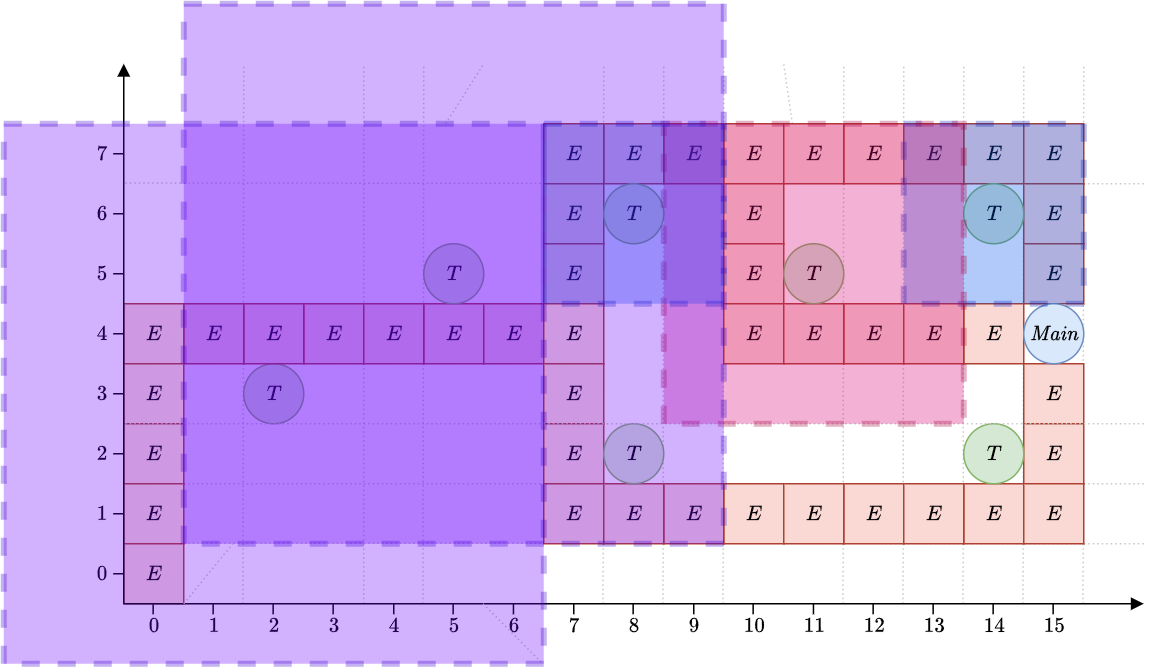
\includegraphics[width=\linewidth]{configs/vanilla/DownFromSnipers.png}
					\caption{\emph{DownFromSnipers} configuration}
				\end{minipage}
			\end{figure}
			\begin{figure}[h!]
				\centering
				\begin{minipage}{.4\textwidth}
					\centering
					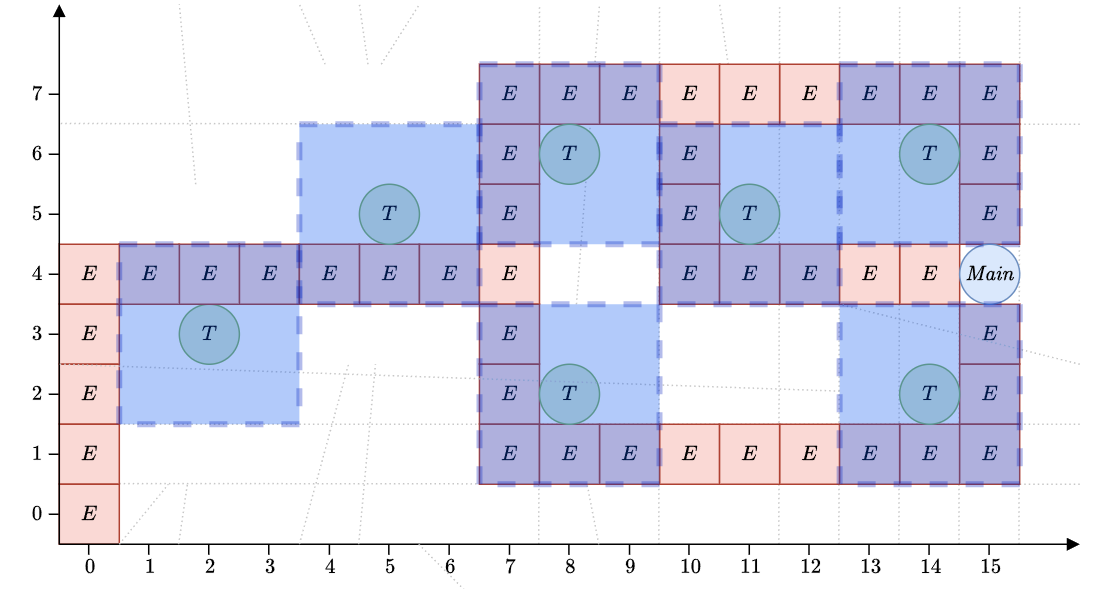
\includegraphics[width=\linewidth]{configs/vanilla/Cannonphobia.png}
					\caption{\emph{Cannonphobia} configuration}
				\end{minipage}
				\begin{minipage}{.5\textwidth}
					\centering
					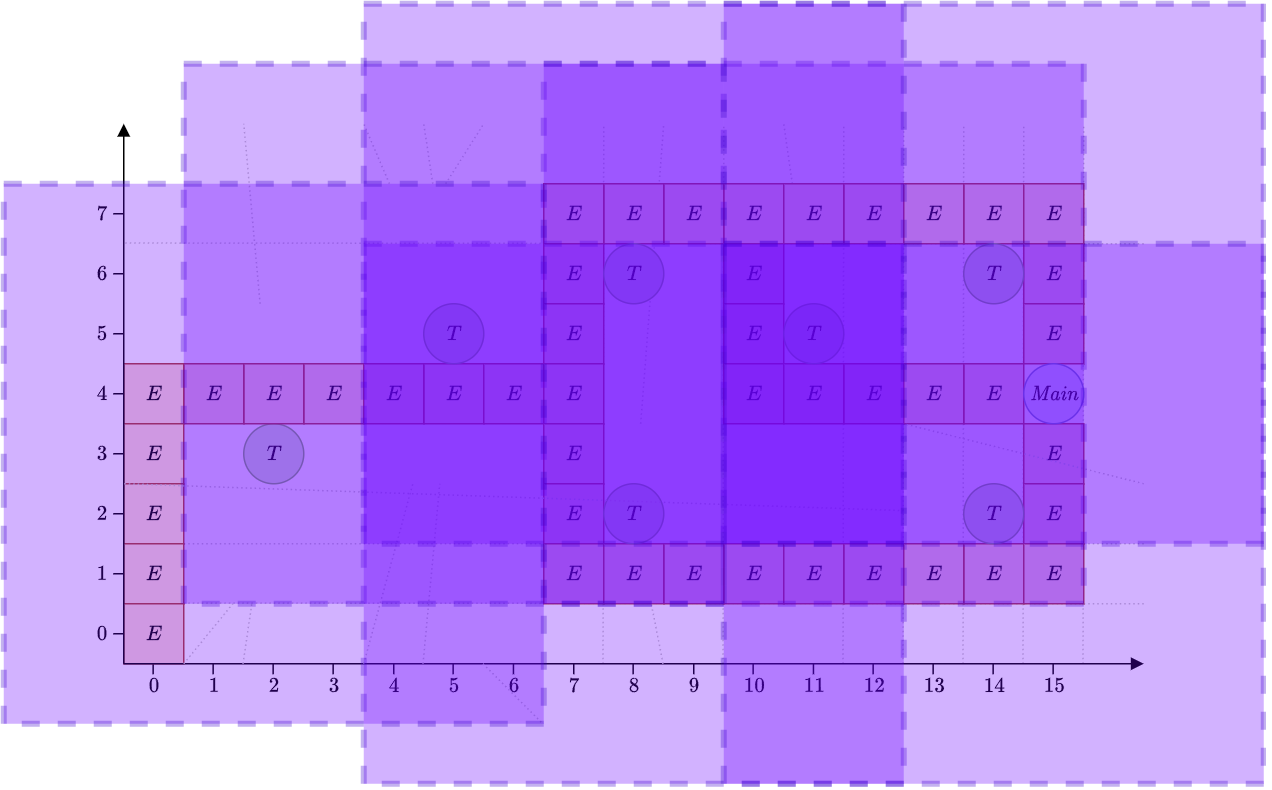
\includegraphics[width=\linewidth]{configs/vanilla/Sniperphobia.png}
					\caption{\emph{Sniperphobia} configuration}
				\end{minipage}
			\end{figure}

			First we analyzed if they are winning and of which kind:
			\begin{table}[h!]
				\centering
				\begin{tabularx}{\textwidth}{||X|>{\raggedright\arraybackslash}X|>{\raggedright\arraybackslash}X|>{\raggedright\arraybackslash}X|>{\raggedright\arraybackslash}X||}
					\hline
					& Winning [T/F] & Weakly-winning [T/F] & Strongly-winning [T/F] & Weakly-strongly-winning [T/F] \\
					\hline
					Default 		& T & T & F & T \\ \hline
					DownFromCannons & F & T & F & T \\ \hline
					DownFromSnipers & F & T & F & T \\ \hline
					Cannonphobia 	& T & T & F & T \\ \hline
					Sniperphobia 	& T & T & T & T \\ \hline
				\end{tabularx}
				\caption{Vanilla chosen configurations winning overview}
			\end{table}
			
			Then (mainly to strain more the model and to explore the Uppaal query syntax), we also wanted to define these metrics to evaluate the "strength" of a configuration (we assume that, like in Uppaal, a boolean predicate is evaluated as $1$ if it is \emph{true}, $0$ otherwise):
			\begin{itemize}
				\item \emph{ADMT} (\emph{Average Distance from MT}) : it is the minimum average distance that enemies can have to the MT:
				\begin{center}
					$ADMT:=\min\{\frac{\sum_{e:Enemy} dist(e.pos,MAIN\_POS)}{MAX\_ENEMIES}\}$
				\end{center}
				\item \emph{SE} (\emph{Survived Enemies}) : it is the maximum number of enemies that still were never be killed throughout the whole match:
				\begin{center}
					$SE:=\max\limits_{matchEnded}\{\sum_{e:Enemy} (e.health>0)\}$
				\end{center}
				\item \emph{CUPE} (\emph{Completed Upper Paths Enemies}) : it is the maximum number of enemies that reached the MT by choosing "up" in the junction \{7,4\}:
				\begin{center}
					$CUPE:=\max\{\sum_{e:Enemy} ((e.pos == MAIN\_POS)*(e.chosenPath\neq 2))\}$
				\end{center}
				\item \emph{CLPE} (\emph{Completed Lower Paths Enemies}) : it is the maximum number of enemies that reached the MT by choosing "down" in the junction \{7,4\}:
				\begin{center}
					$CLPE:=\max\{\sum_{e:Enemy} ((e.pos == MAIN\_POS)*(e.chosenPath=2))\}$
				\end{center}
			\end{itemize}
			
			\begin{table}[h!]
				\centering
				\begin{tabular}{||l|c|c|c|c||}
					\hline
					& ADMT & SE & CUPE & CLPE \\
					\hline
					Default 		& 4 & 2 & 2 & 1 \\ \hline
					DownFromCannons & 1 & 5 & 2 & 5 \\ \hline
					DownFromSnipers & 0 & 6 & 2 & 6 \\ \hline
					Cannonphobia 	& 4 & 2 & 2 & 2 \\ \hline
					Sniperphobia 	& 7 & 0 & 0 & 0 \\ \hline
				\end{tabular}
				\caption{Vanilla chosen configurations performances}
			\end{table}
			Note that:
			\begin{itemize}
				\item strongly-winning configurations have a SE of 0 (if an enemy has survived it means that it shot the MT, and so the configuration can't be strongly-winning);
				\item weakly-winning configurations are likely to have lower ADMT since at least of the execution where the MT is defeat, an amount of enemies must arrive at in the MT spot and for the same reason, they are more likely to have higher SE;
				\item is quite unlikely to have a configuration where $CUPE>SE$ or $CLPE>SE$, because enemies that reached the MT are really likely to survive (and they will survive of course in configurations like Cannonphobia where the MT spot is outside of any shooting range).
			\end{itemize}
			At the end, to judge a configuration we may look for the one with an higher ADMT and a lower SE. CUPE and CLPE and are not better than SE to compare configurations, we defined them to demonstrate that configurations that do not cover parts of the map are more like to see (from the MT spot point of view) enemies coming from those parts. Indeed, DownFromCannons and DownFromSnipers have $CUPE\leq CLPE$ since they cover more the higher paths of the map, while more "uniform" configurations tend to have $CUPE=CLPE=SE$ (that holds also from a probabilistic point of view; see the section dedicated to the spawn strategy).
		\subsection{Stochastic version}
			In this section, we present the most interesting results we obtained by analyzing the following parameters in the stochastic version of the game:
			\begin{itemize}
				\item the number of enemies survived;
				\item \emph{ADT} (Average Death Time) : the average time unit in which killed enemies were killed;
				\item \emph{ADD} (Average Death Distance) : the average distance from MT that killed enemies had when they were killed;
				\item MT life.
			\end{itemize}
			in four different configurations (Default, DownFromSnipers, Cannonphobia and Sniperphobia). We also analyzed how they change (if they change significantly) when turrets and enemies parameters are changed.
			
			
			The complete set of plots we generated can be downloaded in EPS (Encapsulated PostScript) and PNG (Portable Network Graphic) formats at \href{https://jmp.sh/0LxAWLjY}{this} shared folder on Jumpshare.
			
			The first interesting result we obtained from the analysis is how the number of survived enemies changes between the configurations:
			\begin{figure}[h!]
				\centering
				\begin{minipage}{.4\textwidth}
					\centering
					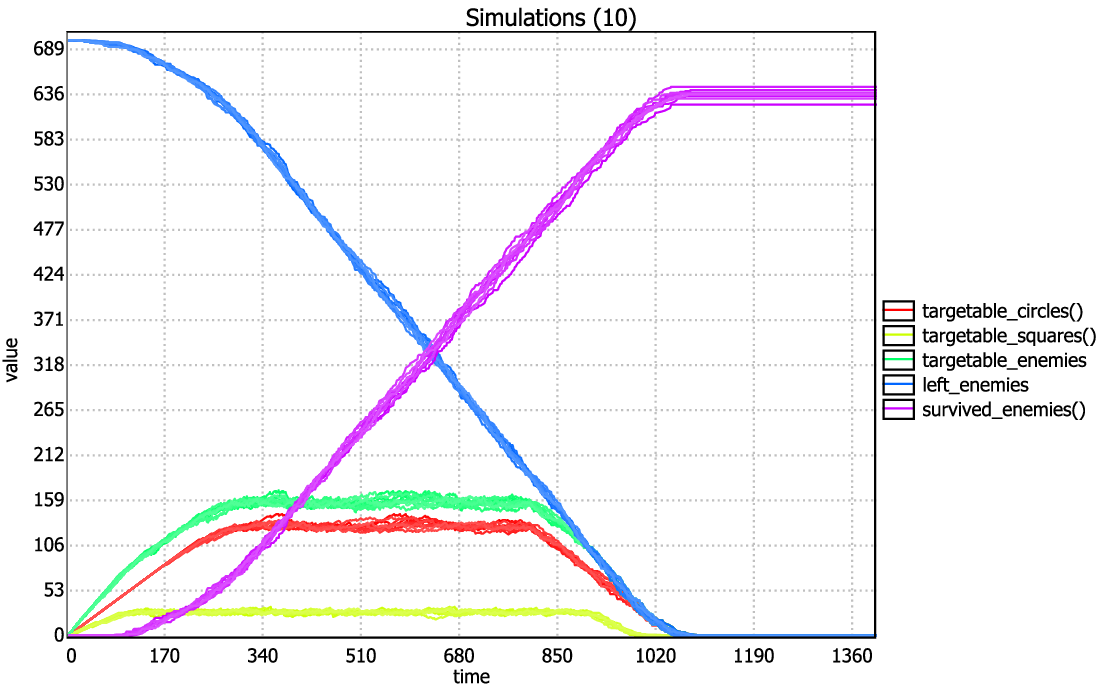
\includegraphics[width=\linewidth]{plots/SE/OVERVIEW WITH 10 RUNS/SNIPERPHOBIA.png}
					\caption{Sniperphobia SE simulation with 10 runs}
				\end{minipage}
				\begin{minipage}{.4\textwidth}
					\centering
					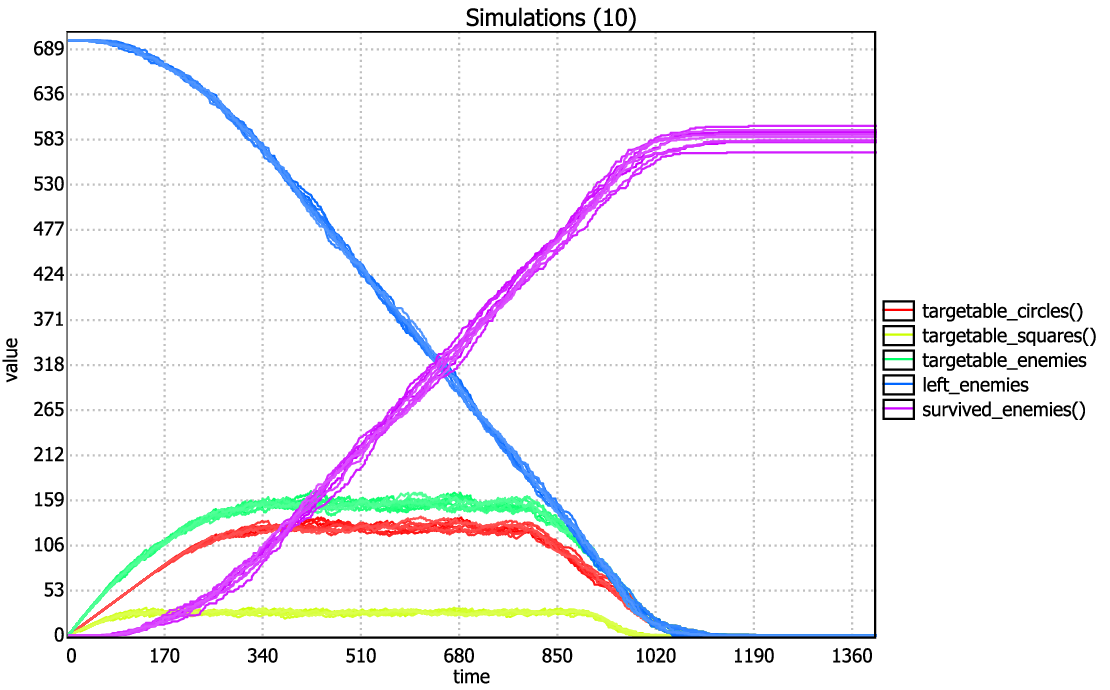
\includegraphics[width=\linewidth]{plots/SE/OVERVIEW WITH 10 RUNS/DOWNFROMSNIPERS.png}
					\caption{DownFromSnipers SE simulation with 10 runs}
				\end{minipage}
			\end{figure}
			\begin{figure}[h!]
				\centering
				\begin{minipage}{.4\textwidth}
					\centering
					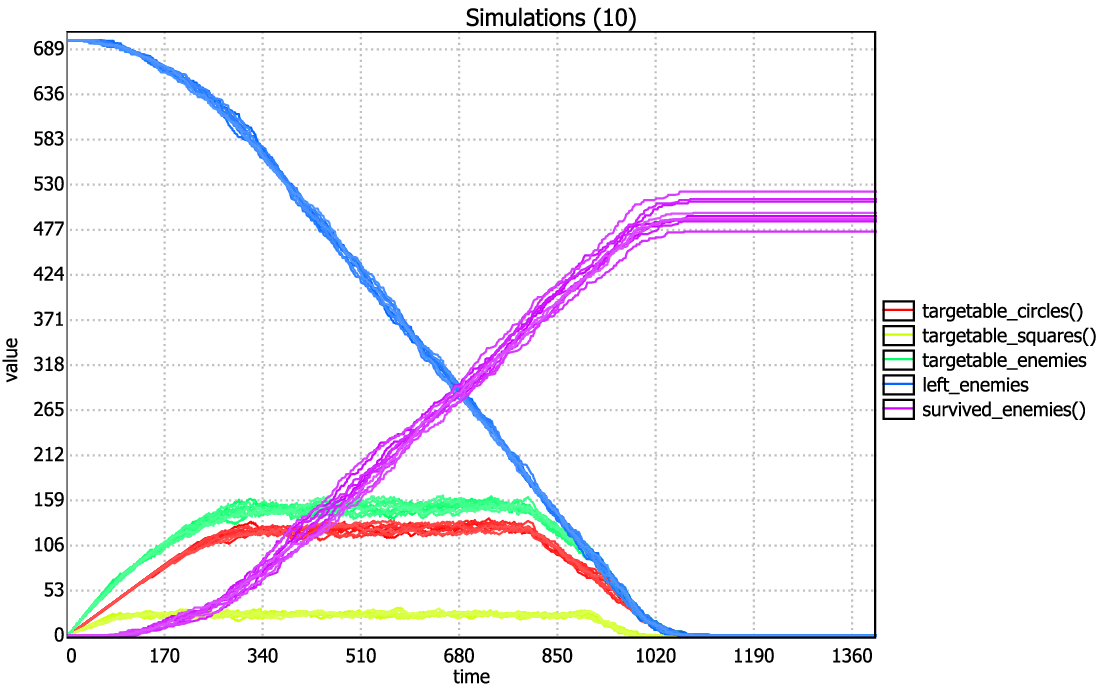
\includegraphics[width=\linewidth]{plots/SE/OVERVIEW WITH 10 RUNS/CANNONPHOBIA.png}
					\caption{Cannonphobia SE simulation with 10 runs}
				\end{minipage}
				\begin{minipage}{.4\textwidth}
					\centering
					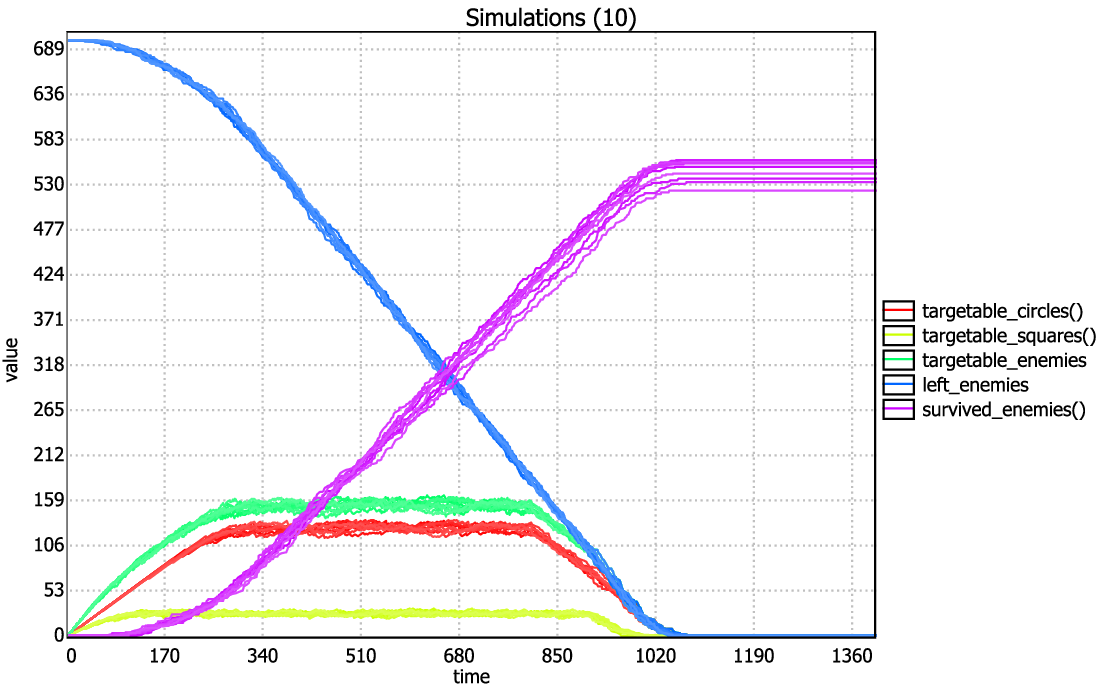
\includegraphics[width=\linewidth]{plots/SE/OVERVIEW WITH 10 RUNS/DEFAULT.png}
					\caption{Default SE simulation with 10 runs}
				\end{minipage}
			\end{figure}
			
			Sniperphobia, which was (the only) strongly-winning configuration in the Vanilla version tends to have a worse SE than the others (even worse than DownFromSnipers which was a weakly-winning configuration).
			However, if we analyze the probability distribution of the SE in first $100$ time units we see better performances with winning and strongly-winning configurations:
			\begin{figure}[h!]
				\centering
				\begin{minipage}{.4\textwidth}
					\centering
					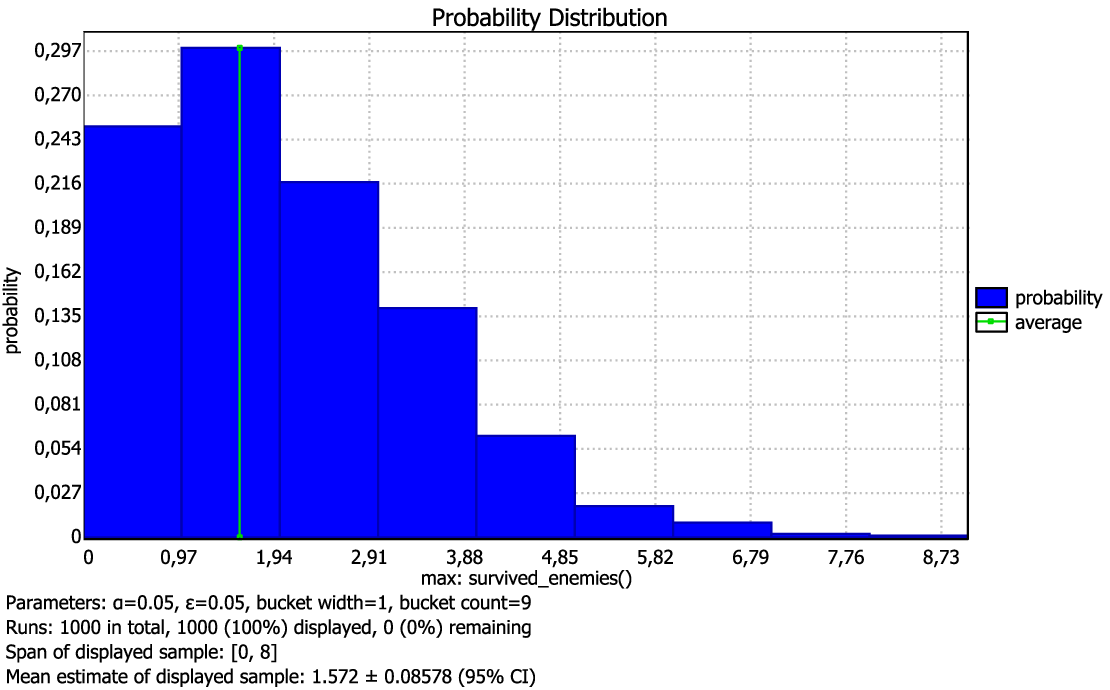
\includegraphics[width=\linewidth]{plots/SE/CLOSE-UP WITH TINY WINDOW/SNIPERPHOBIA.png}
					\caption{Sniperphobia SE probability distribution in the first 100 time units with 1000 runs}
				\end{minipage}
				\begin{minipage}{.4\textwidth}
					\centering
					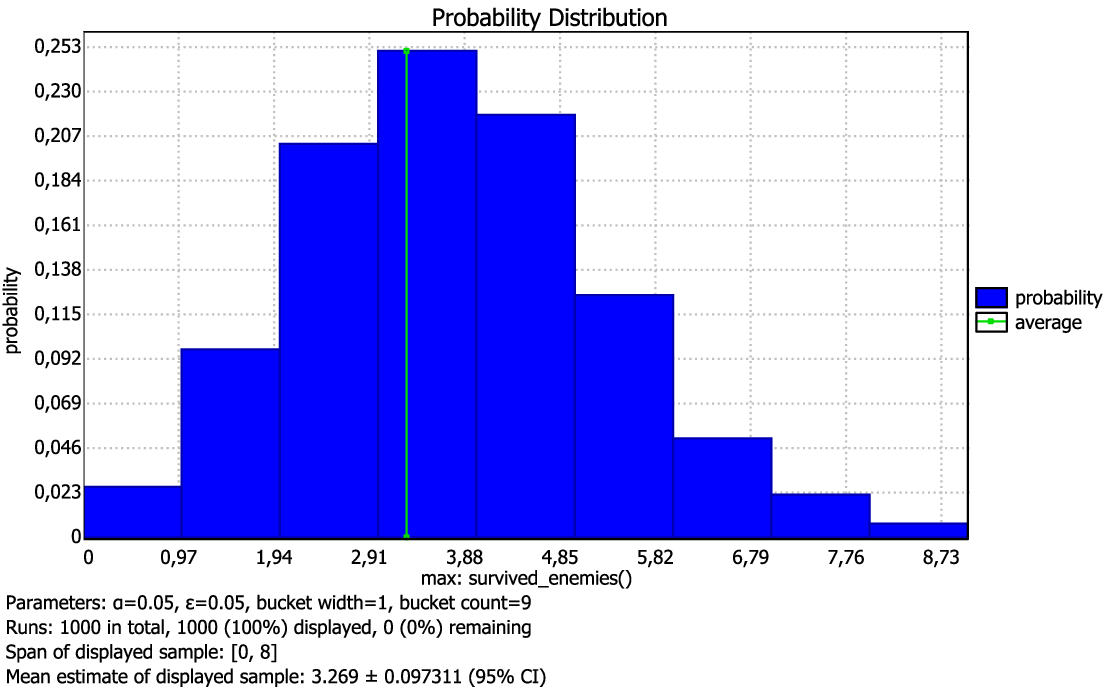
\includegraphics[width=\linewidth]{plots/SE/CLOSE-UP WITH TINY WINDOW/DOWNFROMSNIPERS.png}
					\caption{DownFromSnipers SE probability distribution in the first 100 time units with 1000 runs}
				\end{minipage}
			\end{figure}
			\begin{figure}[h!]
				\centering
				\begin{minipage}{.4\textwidth}
					\centering
					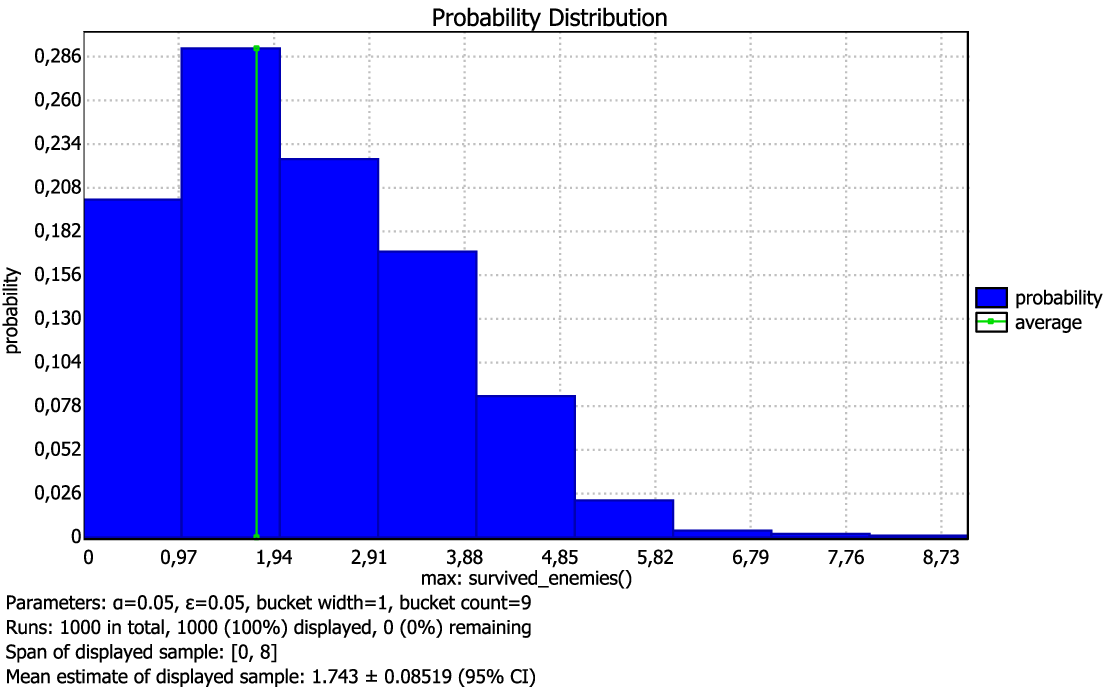
\includegraphics[width=\linewidth]{plots/SE/CLOSE-UP WITH TINY WINDOW/CANNONPHOBIA.png}
					\caption{Cannonphobia SE probability distribution in the first 100 time units with 1000 runs}
				\end{minipage}
				\begin{minipage}{.4\textwidth}
					\centering
					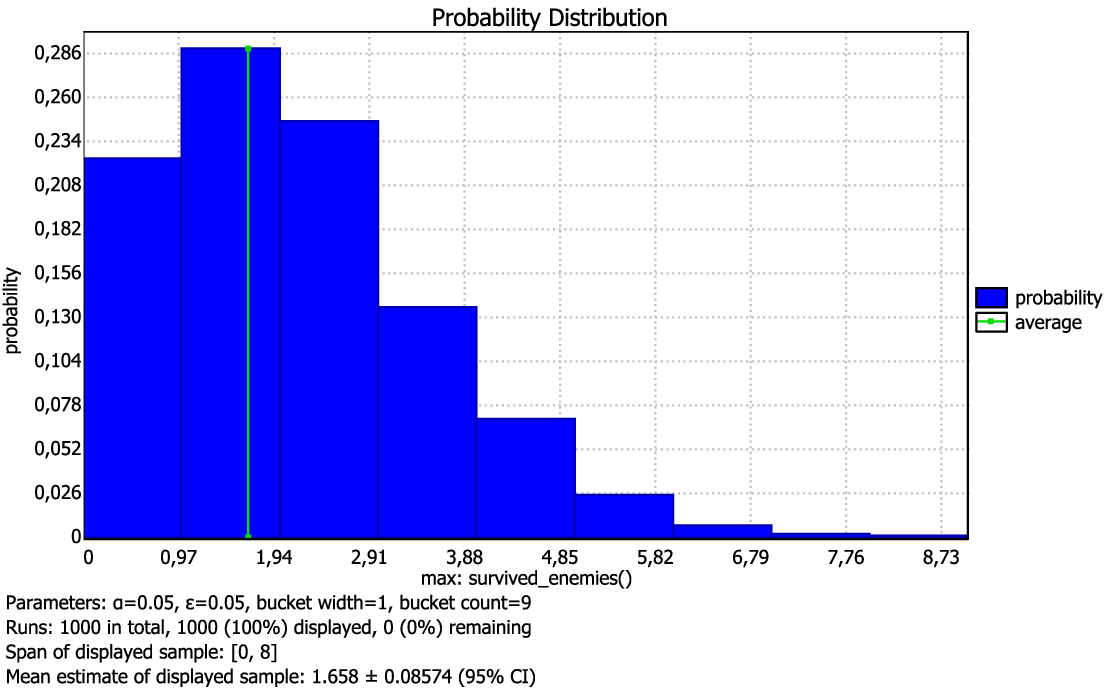
\includegraphics[width=\linewidth]{plots/SE/CLOSE-UP WITH TINY WINDOW/DEFAULT.png}
					\caption{Default SE probability distribution in the first 100 time units with 1000 runs}
				\end{minipage}
			\end{figure}
			Here we see that Sniperphobia tends to have a slight better average value (for SE, the lower the better) than the other configurations and DownFromSnipers is by far the worst one.
			
			Our explanation is that with a large amount of enemies, turrets with higher delays (i.e. snipers compared with cannons) generally tend to have the worse performances. In fact, if we take the delay of snipers down of 7:
			\begin{figure}[h!]
				\centering
				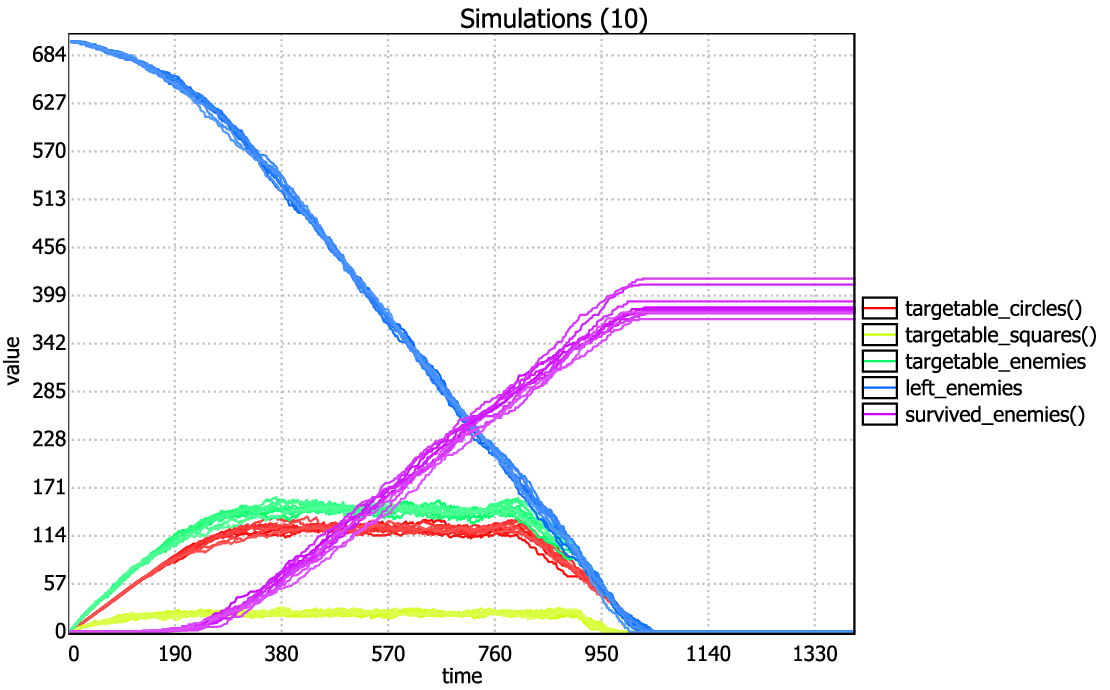
\includegraphics[width=.5\textwidth]{plots/SE/OVERVIEW WITH DELAY 7 SNIPERS/SNIPERPHOBIA.png}
				\caption{Sniperphobia SE simulation with 10 runs (snipers delay set to 7)}
			\end{figure}
			Sniperphobia outclasses any other configuration.
			
			We wanted to present this kind of unexpected behaviors (i.e. strongly-winning configurations may have a worse SE with large waves) not only to show the trivial evidence that the lower turret delay, the better performances, but also to show that stochastic model checking can reveal behaviors that with exhaustive model checking would have been too heavily computationally complex to verify. With stochastic model checking we were able to show that in larger waves, a turret with a lower damage but a lower firing speed tends to provide better performances over turrets with higher damages and higher speeds.
			
			While analysis of ADT and MT life have not really shown surprising results respect to the ones shown with the analysis of the SE (mettere spiegazione), a curious result came from the analysis of the ADD, in particular:
			\begin{figure}[h!]
				\centering
				\begin{minipage}{.4\textwidth}
					\centering
					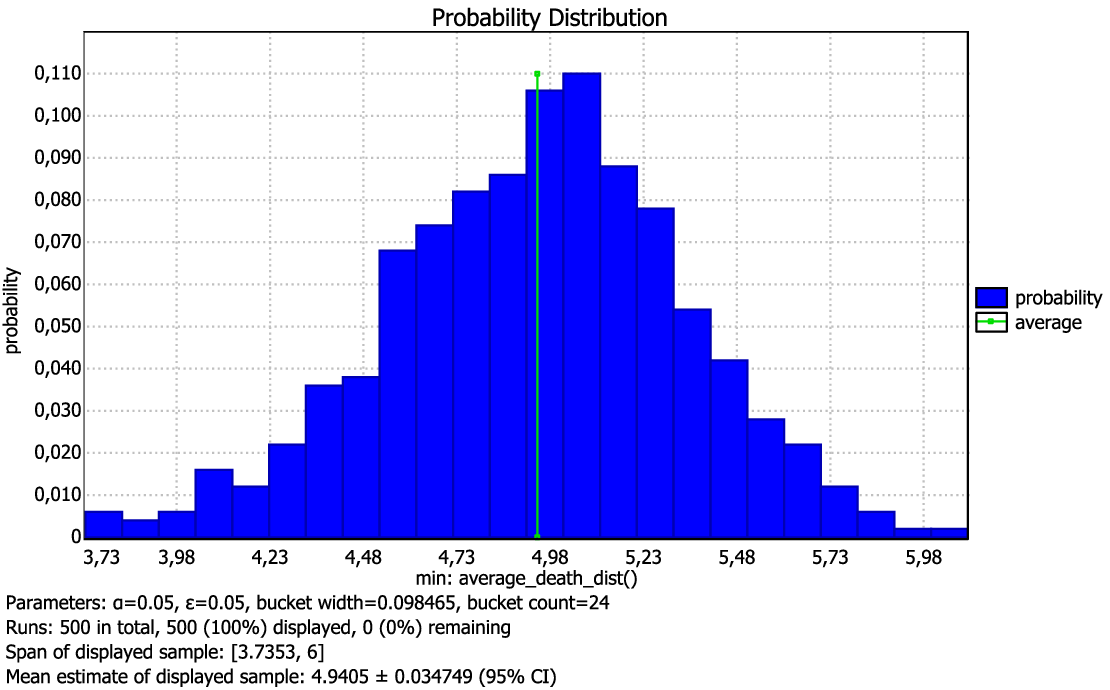
\includegraphics[width=\linewidth]{plots/ADD/PD/SNIPERPHOBIA.png}
					\caption{Cannonphobia ADD probability distribution in the first 100 time units with 500 runs}
				\end{minipage}
				\begin{minipage}{.4\textwidth}
					\centering
					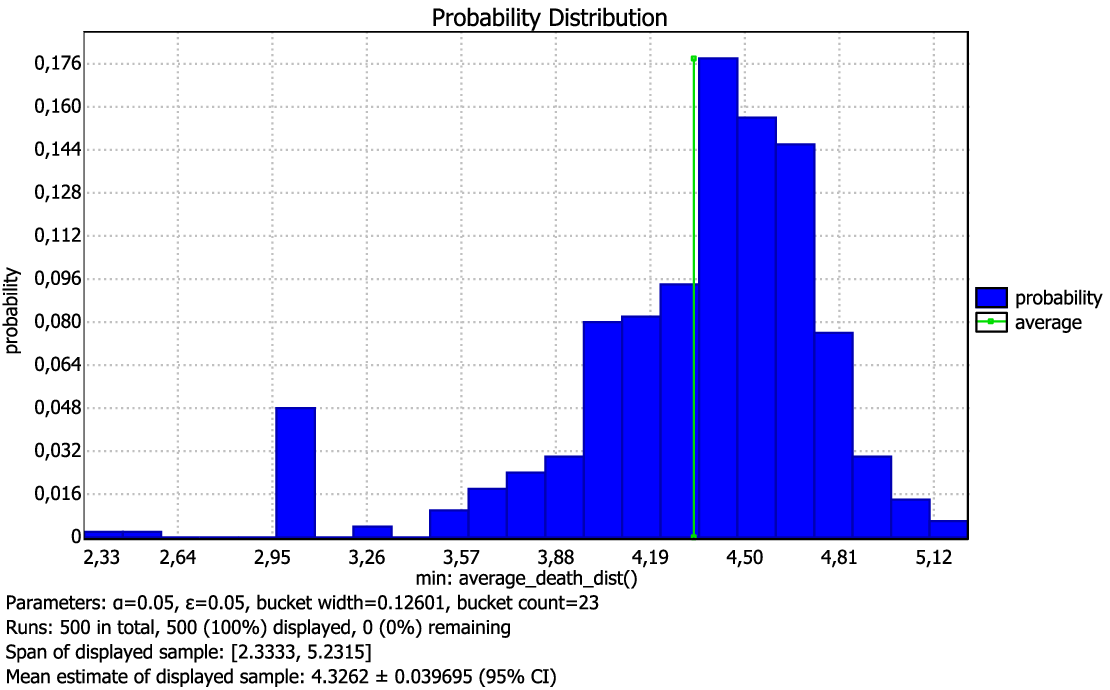
\includegraphics[width=\linewidth]{plots/ADD/PD/DOWNFROMSNIPERS.png}
					\caption{DownFromSnipers ADD probability distribution in the first 100 time units with 500 runs}
				\end{minipage}
			\end{figure}
			\begin{figure}[h!]
				\centering
				\begin{minipage}{.4\textwidth}
					\centering
					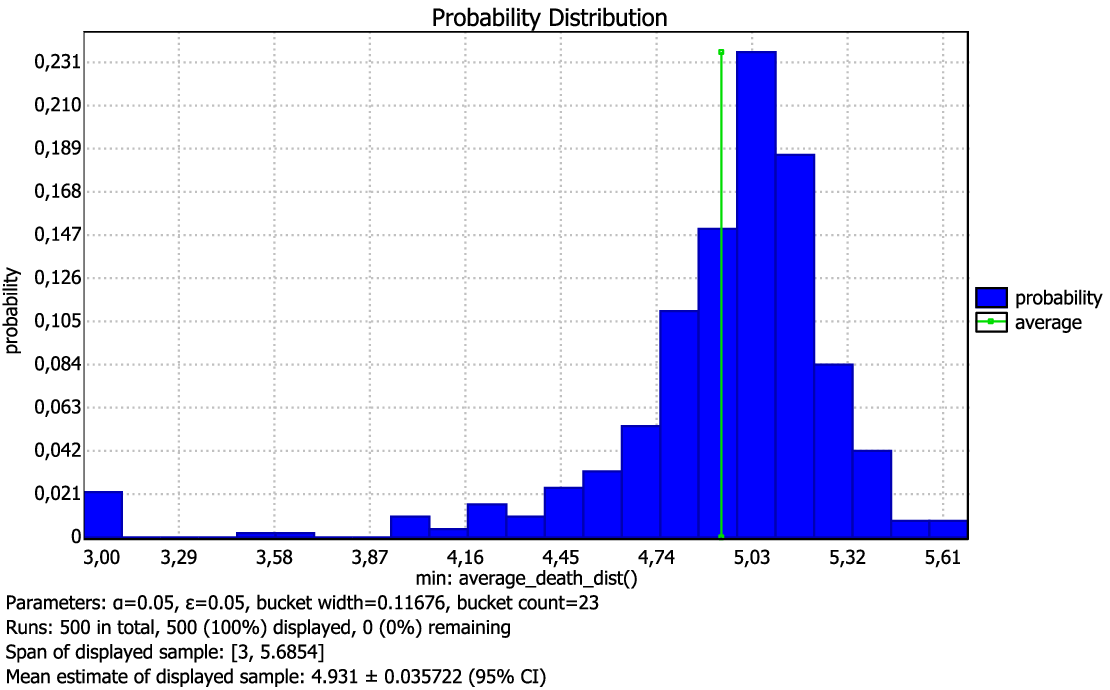
\includegraphics[width=\linewidth]{plots/ADD/PD/CANNONPHOBIA.png}
					\caption{Cannonphobia ADD probability distribution in the first 100 time units with 500 runs}
				\end{minipage}
				\begin{minipage}{.4\textwidth}
					\centering
					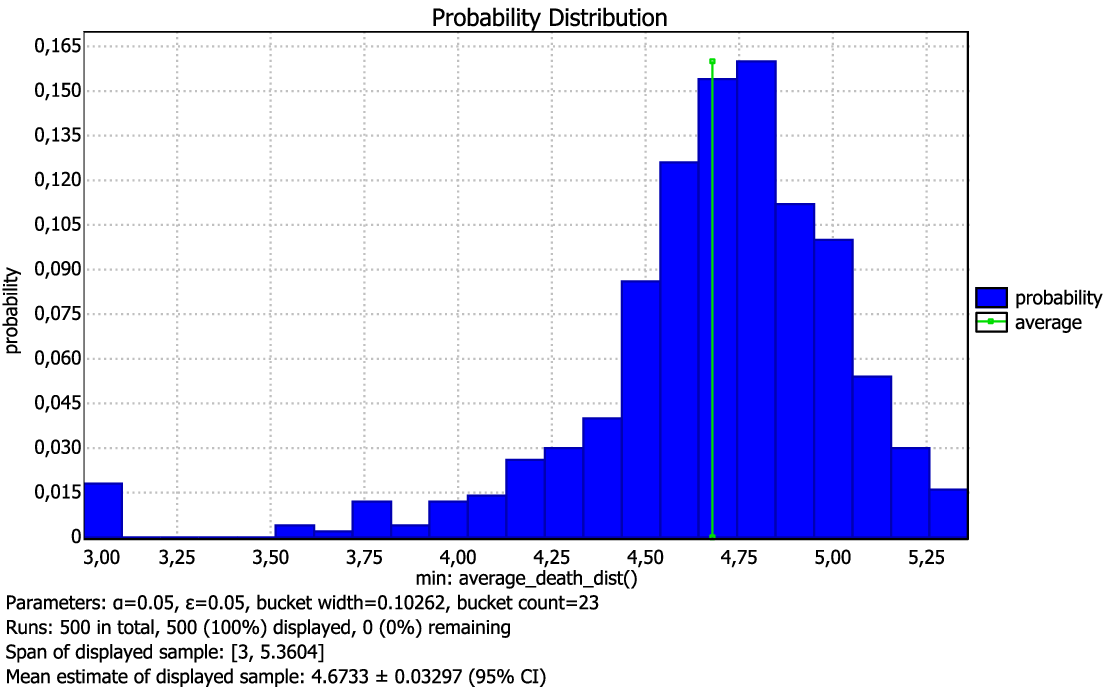
\includegraphics[width=\linewidth]{plots/ADD/PD/DEFAULT.png}
					\caption{Default ADD probability distribution in the first 100 time units with 500 runs}
				\end{minipage}
			\end{figure}
			Finally, we simulated the system in what we may call the \emph{Over Range mode}: any turret has a range of 15 (i.e. any turret may fire enemies in any point of the map). We may think that is parameter choice tends to uniform the performances or to let snipers to outclass cannons and basic however, no index changed significantly its trend also in comparison to the ones of other configurations. The only notable change we found is that ADD tends to have a more hyperbolic shape:
			\begin{figure}[h!]
				\centering
				\begin{minipage}{.4\textwidth}
					\centering
					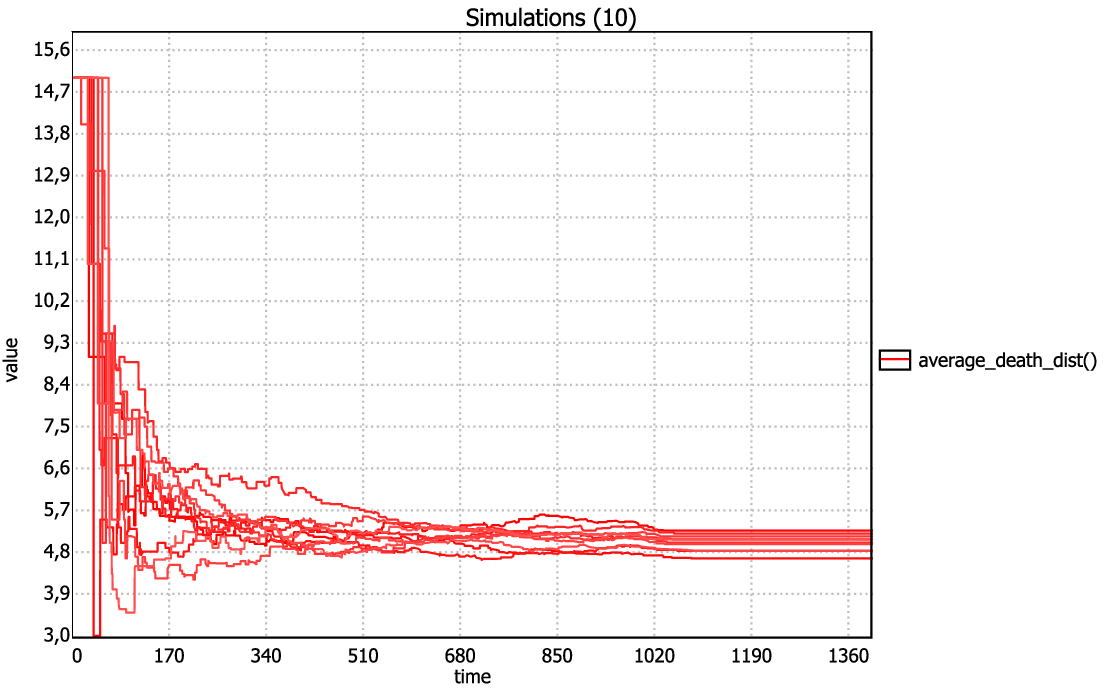
\includegraphics[width=\linewidth]{plots/ADD/OVERVIEW WITH 10 RUNS/CANNONPHOBIA.png}
					\caption{Cannonphobia ADD simulation with 10 runs}
				\end{minipage}
				\begin{minipage}{.4\textwidth}
					\centering
					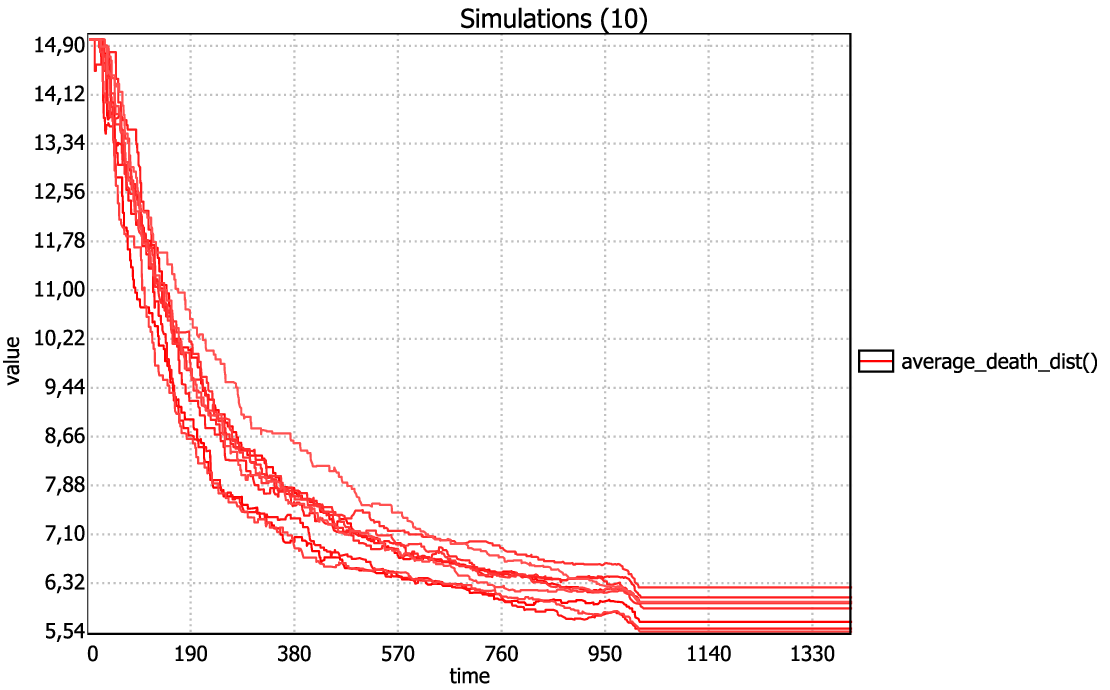
\includegraphics[width=\linewidth]{plots/ADD/OVERVIEW WITH OVER RANGE/CANNONPHOBIA.png}
					\caption{Cannonphobia ADD simulation with 10 runs (in over range mode)}
				\end{minipage}
			\end{figure}
			\begin{figure}[h!]
				\centering
				\begin{minipage}{.4\textwidth}
					\centering
					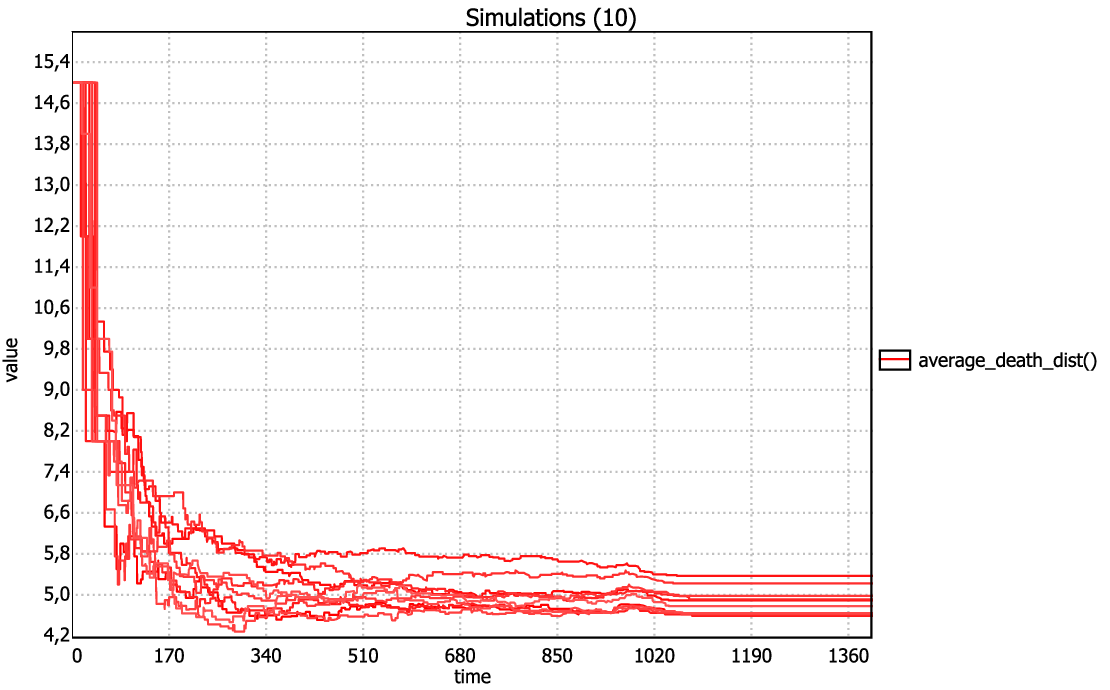
\includegraphics[width=\linewidth]{plots/ADD/OVERVIEW WITH 10 RUNS/DEFAULT.png}
					\caption{Default ADD simulation with 10 runs}
				\end{minipage}
				\begin{minipage}{.4\textwidth}
					\centering
					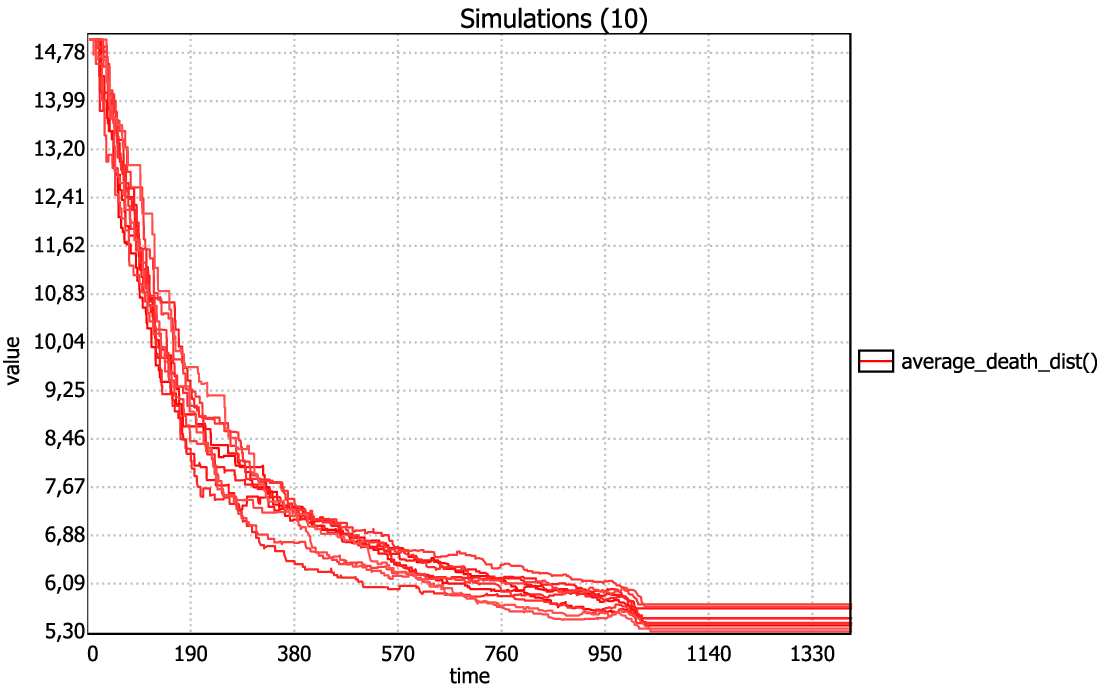
\includegraphics[width=\linewidth]{plots/ADD/OVERVIEW WITH OVER RANGE/DEFAULT.png}
					\caption{Default ADD simulation with 10 runs (in over range mode)}
				\end{minipage}
			\end{figure}
			In other words, the product between the ADD and the time tends to be constant.
	\section{Conclusions}
		Conclusions.
	\newpage
	\appendix
	\section{Discarded choices}
		We wanted to write this additional section mainly to better clarify the reasons behind our final design choices. Nonetheless, we would like to clarify that our design choices are what we believed to be more efficient and adequate for our interpretation of the game, so some of the discarded can possibly be the best ones in other contexts or with different requirements and also for this reason we wanted to state them in the report.
		\subsection{MT template}
			Originally, a template for MT was designed. It was, for its simplicity, the very first one to be designed (\texttt{decDamage} decreases MT's life by the value set in a global variable from the firing enemy):
			
			\begin{figure}[h!]
				\centering
				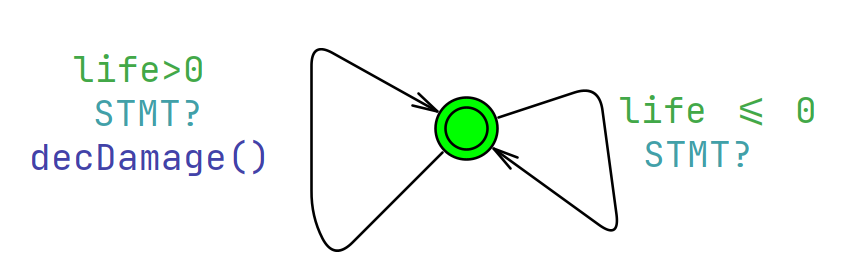
\includegraphics[width=0.5\textwidth]{MT_Template.png}
				\caption{Original MT's template}
			\end{figure}
		\subsection{Hard-coded enemies paths}
			The very first enemy version used the concept of \texttt{next} but there was no idea on how to model the non-deterministic moves (unless using function \texttt{random}, which is not available in symbolic simulation). The only idea was to hard-code vectors of cells representing each straight red path on the map and enemies template would have chosen between them non-deterministically with transitions (once an enemy arrives in the last cell of a path, then it will start to follow non-deterministically one of the "next paths"):
			
			\begin{figure}[h!]
				\centering
				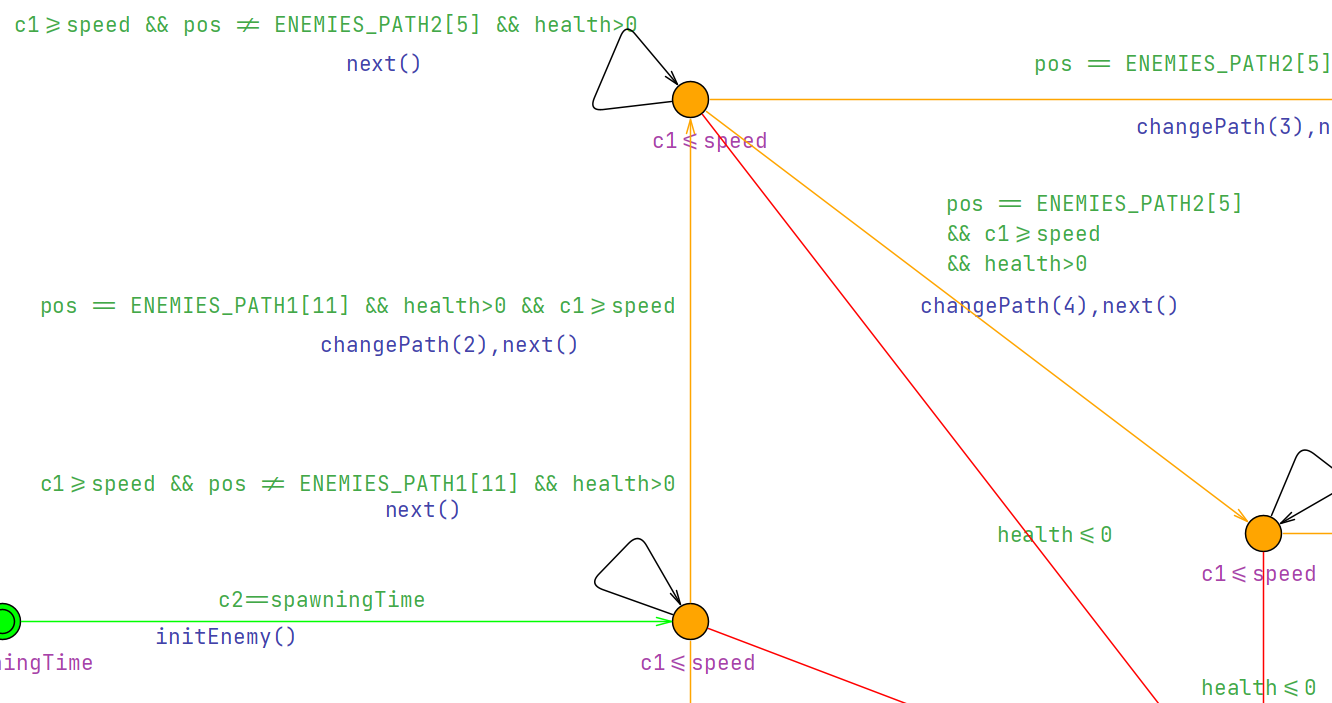
\includegraphics[width=0.65\textwidth]{ENEMIES_PATHS.png}
				\caption{Original non-deterministic path choices example}
			\end{figure}
		\subsection{Quadratic enemies scanning strategy}
			The very first turret version used to look for enemies to shoot in this way: for each $k$ from $1$ to the \texttt{range}, scan \texttt{SHOOT\_TABLE} to find all the available enemies at exactly $k$ cells of distance; then, choose the best iso-distant available enemy based on the requirements criteria. The worst-case asymptotic complexity of this procedure was $\Theta(k\times MAX\_ENEMIES)$ which was significantly worse than the one of the final version which is $\Theta(MAX\_ENEMIES)$ especially in the average case where there is no enemy inside the shooting range.
		\subsection{Locks}
			At the beginning, the first way of synchronizing entities was thought in a classical lock-unlock manner:
			\begin{figure}[h!]
				\centering
				\begin{minipage}{.5\textwidth}
					\centering
					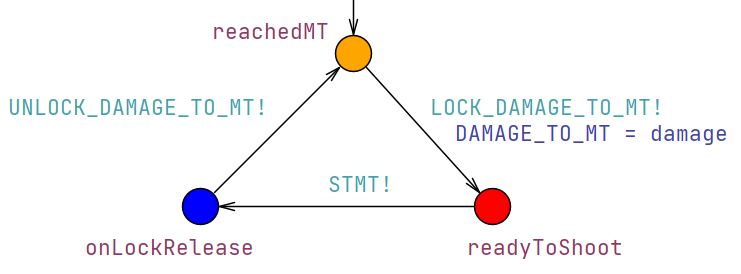
\includegraphics[width=.9\linewidth]{enemyLock.png}
					\caption{Close-up of the enemy locking \texttt{STMT} channel}
				\end{minipage}
				\begin{minipage}{.4\textwidth}
					\centering
					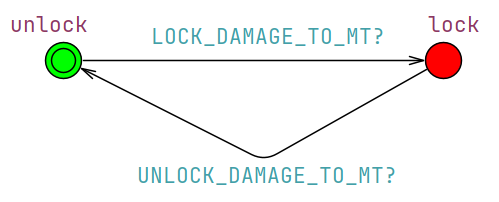
\includegraphics[width=.9\linewidth]{controller.png}
					\caption{\texttt{STMTCONTROLLER} template}
				\end{minipage}
			\end{figure}
			Once an enemy reaches the MT (for the MT template please see the proper section of the appendix):
			\begin{enumerate}
				\item the enemy sends a message to \texttt{STMTCONTROLLER} and waits for its reply (more precisely, Uppaal chooses non-deterministically which one of the ready enemies can send the message to the controller);
				\item once the controller replies the enemy places in the shared variable the damage for the MT;
				\item the enemy shoots to the MT (i.e. sends a message over \texttt{STMT});
				\item the enemy sends a message to \texttt{STMTCONTROLLER} to release the "lock".
			\end{enumerate}
			We understand that this solution is:
			\begin{itemize}
				\item deadlock-free: soon or later an acquired lock will be released and soon or later a lock request will be accepted;
				\item not starvation-free: since it is not guaranteed that any enemy that requests a lock will eventually obtain it.
			\end{itemize}
			We removed this concept since we understood that a single transition that both changes the global variable and performs the shoot would have produced the same behavior, since, provided that this transition is not synchronized with other enemies, only one of them can perform it in a time instant, therefore there is no possibility that an enemy places the damage for the MT into the shared variable and before sending the shooting message another enemy changes the variable and (or not) shoots to the MT (which would clearly create an undesired behavior).
		\subsection{Lifetime counter}
			As we have seen, turrets understand that an enemy is present on the map for a shorter amount of time by looking to its spawning. This idea lets enemies to not keep a counter updated to tell the turrets that they are present on the map for tot. time units. However, this idea is relatively new in the history of the model, since at the beginning, the lifetime of an enemy used to be update in each time unit by the enemy:
			
			\begin{figure}[h!]
				\centering
				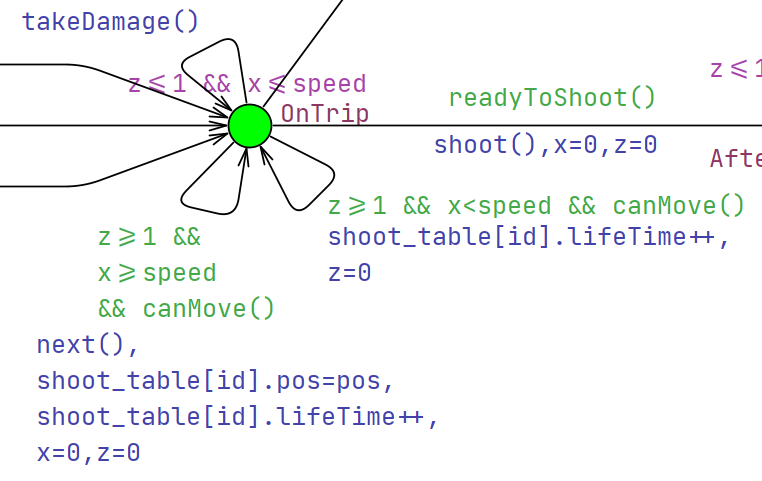
\includegraphics[width=0.5\textwidth]{lifetimeCounter.png}
				\caption{Close-up of of the lifetime counter of an enemy}
			\end{figure}
			With clock \texttt{z} at each time unit the lifetime counter would have been updated.
			
			Note that this solution was also used to verify that enemies would have reached the MT spot in no more than $\texttt{MAX\_PATH\_LENGTH}\times speed$ time units.
	\nocite{1,2,3,4,5,6,7}
	\printbibliography
\end{document}